\documentclass{article}

% Set page size and margins
% Replace `letterpaper' with `a4paper' for UK/EU standard size
\usepackage[letterpaper,top=2cm,bottom=2cm,left=3cm,right=3cm,marginparwidth=1.75cm]{geometry}
\usepackage[spanish]{babel}
\usepackage{url}
\usepackage{hyperref}
\usepackage{csquotes}
\usepackage{amsmath}
\usepackage{amssymb}
\usepackage{graphicx}
\usepackage{listings}
\usepackage{xcolor}
\usepackage{setspace}
\usepackage{float}

\graphicspath{ {assets/} }

%Code colors:
\definecolor{codegreen}{rgb}{0,0.6,0}
\definecolor{codegray}{rgb}{0.5,0.5,0.5}
\definecolor{codepurple}{rgb}{0.58,0,0.82}
\definecolor{backcolour}{rgb}{0.95,0.95,0.92}
\doublespacing

\lstdefinestyle{mystyle}{
    backgroundcolor=\color{backcolour},
    commentstyle=\color{codegreen},
    keywordstyle=\color{magenta},
    numberstyle=\tiny\color{codegray},
    stringstyle=\color{codepurple},
    basicstyle=\ttfamily\footnotesize,
    breakatwhitespace=false,
    breaklines=false,
    captionpos=b,
    keepspaces=true,
    numbers=left,
    numbersep=5pt,
    showstringspaces=false,
    showlines=false,
    showtabs=false,
    tabsize=2
}

\lstset{style=mystyle}

\NewDocumentCommand{\codeword}{v}{%
    \texttt{\textcolor{black}{#1}}%
}

\begin{document}

    \begin{titlepage}
        \centering
        {
\includegraphics[width=0.5\textwidth]{logo2}\par}
        {\bfseries\LARGE Universidad Católica del Uruguay \par}
        \vspace{0.3cm}
        {\scshape\Large Facultad de Ingeniería \par}
        \vspace{0.3cm}
        {\scshape\Huge Proyecto - Lights Out!\par}
        \vspace{1cm}
        {\Large Álgebra Aplicada \par}
        {\Large Profesor: Maglis Mujica \par}
        \vfill
        {\Large Autores: \par}
        {\Large Piero Saucedo (5.342.503-5)\\Juan Martín Riccetto (5.324.939-0)\\Juan Manuel Pérez (4.673.899-0) \par}
        \vfill
        {\Large \today \par}
    \end{titlepage}

    \section{Introducción}\label{sec:introduccion}
    En el marco teórico de Álgebra Aplicada, se propone a los estudiantes una tarea centrada en el uso de sistemas de ecuaciones.

    En esta ocasión, el objetivo principal se trata de estudiar el juego electrónico "Lights Out!", que consiste en un tablero n×n de luces que pueden estar prendidas o apagadas de forma aleatoria, y el jugador deberá alcanzar un estado en el que todas las luces estén apagadas.
    Se buscará verificar si ciertas variables, como el orden o el número de veces en el que son presionadas las distinas luces son relevantes o no.

    \section{Marco Teórico}

    \subsection{Sistema lineal de ecuaciones}
    Un sistema lineal de m ecuaciones y n incognitas, es un conjunto (S) de ecuaciones de la forma:\\
    \[
        S: \left\{
        \begin{aligned}
            a_{11}x_{11} + \cdots + a_{1n}x_{1n} &= b_1 \\
            \vdots \hspace{3em}\\
            a_{m1}x_{1} + \cdots + a_{mn}x_{n} &= b_m
        \end{aligned}
        \right.
    \]
    \\
    Donde $a_ij$ son los coeficientes, $x_i$ las incógnitas y $b_i$ los términos independientes.\\

    Una solución del sistema, es un conjunto de números reales: $\alpha_1$,...,$\alpha_n$, tales que verifican todas las ecuaciones que conforma el sistema.

    \subsubsection{Clasificación de los sistemas de ecuaciones}
    Existen cuatro formas de clasificar un sistema de ecuaciones:
    \begin{itemize}
        \item \textbf{Compatible:} Si admite alguna solución.
        \item \textbf{Incompatible:} Si no admite solución.
        \item \textbf{Compatible Determinado:} Si admite una única solución.
        \item \textbf{Compatible Indeterminado:} Si admite soluciones infinitas.
    \end{itemize}

    \subsection{Matrices}
    Una \textbf{matriz} es un arreglo bidimensional de números reales o complejos, organizado en $m$ filas y $n$ columnas. Las filas son las líneas horizontales y las columnas son las verticales. Por tanto, el tamaño de una matriz se representa como $m \times n$, donde $m$ es el número de filas y $n$ es el número de columnas.

    \subsection{Matriz cuadrada} Una \textbf{matriz cuadrada} es aquella que tiene el mismo número de filas y columnas, es decir, su tamaño es $n \times n$.

    \subsection{Clasificación de los sistemas de ecuaciones}

    \subsubsection*{Sistema lineal de ecuaciones}
    Un sistema lineal $(S)$ se puede clasificar de la siguiente manera:
    \begin{itemize}
        \item \textbf{Compatible:} Tiene al menos una solución.
        \item \textbf{Incompatible:} No tiene solución.
        \item \textbf{Compatible Determinado:} Tiene una única solución.
        \item \textbf{Compatible Indeterminado:} Tiene infinitas soluciones.
    \end{itemize}
    
    \subsubsection*{Representación matricial de un sistema lineal}
    
    Dado el sistema lineal:
    \[
    S: \left \{
    \begin{array}{@{}l@{}}
    a_{11}x_1 + \dots + a_{1n}x_n = b_1 \\
    \hspace{1.8cm}\vdots\\
    a_{m1}x_1 + \dots + a_{mn}x_n = b_m
    \end{array}
    \right.
    \]
    
    Podemos representarlo en forma matricial como $A.X = b$, donde:
    \[
    A = 
    \begin{pmatrix}
    a_{11}  & \dots & a_{1n}\\
    .       & .     & .\\
    .       & .     & .\\
    .       & .     & .\\
    a_{m1}  & \dots & a_{mn}
    \end{pmatrix}
    \quad
    X = 
    \begin{pmatrix}
    x_1\\
    .\\
    .\\
    .\\
    x_n
    \end{pmatrix}
    \quad
    b = 
    \begin{pmatrix}
    b_1\\
    .\\
    .\\
    .\\
    b_m
    \end{pmatrix}
    \]
    
    Aquí, $A$ es la matriz de coeficientes, $X$ es el vector de incógnitas y $b$ el vector de términos independientes.
    
    \paragraph{Matriz Ampliada}
    
    La matriz ampliada se forma agregando la columna de términos independientes a la matriz de coeficientes:
    \[
    \begin{pmatrix}
    a_{11} & \dots & a_{1n} & b_1 \\
    .      & .     & .      & .   \\
    .      & .     & .      & .   \\
    a_{m1} & \dots & a_{mn} & b_m
    \end{pmatrix}
    \]
    
    \subsubsection*{Sistemas lineales homogéneos}
    
    Un sistema lineal es \textbf{homogéneo} si se expresa como:
    \[
    H: \left \{
    \begin{array}{@{}l@{}}
    a_{11}x_1 + \dots + a_{1n}x_n = 0 \\
    \hspace{1.8cm}\vdots\\
    a_{m1}x_1 + \dots + a_{mn}x_n = 0
    \end{array}
    \right.
    \]
    Este sistema siempre tiene la solución trivial $x_1 = 0,\dots, x_n = 0$. Un sistema homogéneo es siempre compatible y puede ser determinado o indeterminado.
    
    \subsubsection{Sistemas equivalentes}
    
    Dos sistemas de ecuaciones son equivalentes si comparten el mismo conjunto de soluciones.
    \\Ejemplo:
    \[
    S_1: \left \{
    \begin{array}{@{}l@{}}
    2x = 2 \\
    y = 2
    \end{array}
    \right.
    \quad
    S_2: \left \{
    \begin{array}{@{}l@{}}
    x = 1 \\
    y = 2
    \end{array}
    \right.
    \]
    Estos dos sistemas son equivalentes porque tienen las mismas soluciones: $S_1 \sim S_2$, ya que $sol(S_1) = sol(S_2) = (1,2)$.
    
    \subsubsection*{Teorema fundamental de equivalencias de sistemas}
    
    Cualquier transformación elemental realizada en un sistema lineal de ecuaciones genera un sistema equivalente.

    \newpage
    
    \subsection{Método de Gauss}
    
    El método de Gauss permite resolver un sistema de ecuaciones lineales mediante la eliminación de incógnitas. Dado un sistema en forma matricial $Ax = B$, con $A$ la matriz de coeficientes, $x$ el vector de incógnitas, y $B$ el vector de términos independientes, el método se basa en transformar la matriz aumentada $[A|B]$ en una matriz triangular superior. Luego, se utiliza sustitución hacia atrás para obtener las soluciones. Los pasos del método son:
        
    \begin{enumerate}
        \item \textbf{Formar la matriz aumentada}: Se combina la matriz de coeficientes con el vector de términos independientes.
        \item \textbf{Pivoteo}: Si el valor de mayor magnitud en una columna no está en la diagonal, se intercambian filas.
        \item \textbf{Eliminación hacia adelante}: Se aplican operaciones elementales para convertir en cero los elementos debajo de la diagonal principal.
        \item \textbf{Sustitución hacia atrás}: Una vez que se tiene la matriz triangular superior, se resuelven las ecuaciones comenzando por la última fila.
    \end{enumerate}

    \subsection{Lights Out}
    Lights Out es un juego de lógica que consiste en un tablero de \(5 \times 5\) (aunque existen versiones con tableros de diferentes tamaños). Cada celda del tablero contiene una luz que puede estar encendida o apagada. El objetivo del juego es apagar todas las luces del tablero.

    \begin{figure}[h]
        \centering
        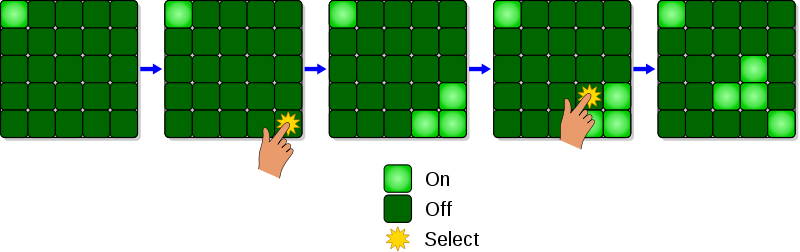
\includegraphics[scale=0.4]{lightsout.png}
    \end{figure}


    \subsubsection*{Reglas del juego}
    Al comenzar, el tablero tiene un patrón aleatorio de luces encendidas y apagadas. El jugador puede pulsar cualquier celda del tablero. Al hacerlo, la luz de esa celda cambia de estado (si está encendida, se apaga; si está apagada, se enciende). Además, las luces adyacentes (arriba, abajo, izquierda y derecha) también cambian de estado.

    El jugador debe continuar presionando celdas hasta que todas las luces del tablero estén apagadas.

    \newpage

    \section{Objetivos}
    El propósito de este proyecto es desarrollar una función en Python que permita analizar una matriz cuadrada de dimensiones \(n \times n\), donde cada elemento puede tomar uno de dos valores: \(0\) o \(1\). Esta matriz representa el estado inicial del juego Lights Out. La función debe implementar el modelo matemático especificado en el documento del proyecto, utilizando este modelo para obtener un vector resultante de unos y ceros que corresponda a la solución del juego.
    
    Para resolver el sistema de ecuaciones asociado al modelo, se requiere adaptar el algoritmo de eliminación gaussiana, teniendo en cuenta que se opera en el conjunto \(\{0, 1\}\) utilizando la suma binaria, sin necesidad de realizar productos.
    
    Este método asegura la eficiencia del proceso, ya que está optimizado para las propiedades específicas del conjunto \(\{0, 1\}\). La función final devolverá el vector solución, lo cual permitirá resolver el juego Lights Out aplicando principios matemáticos adaptados a la naturaleza del problema.

    \newpage

    \section{Desarrollo}
    
    \subsection{¿Es necesario presionar alguna luz más de una vez para resolver el juego?}
    No, no es necesario, ya que las luces solo pueden tener dos estados (encendido y apagado). Si se presiona una luz, cambia su estado y el de sus vecinos; pero si se vuelve a presionar la misma luz, el cambio se revierte, retornando las luces a su estado original.
    
    \subsection{¿Importa el orden en que se presionan las luces para obtener la solución?}
    
    El orden no es relevante. Como el estado de una luz afecta también a sus vecinas, se puede llegar al mismo resultado sin importar el orden en que las luces sean presionadas.

    \subsection{Justificación de por qué el modelo matemático es adecuado para resolver el juego}

    El estado de cada casilla del tablero, encendida o apagada, se puede representar utilizando el conjunto $\mathbb{Z}_2$, que corresponde a los enteros módulo 2, es decir, el conjunto $\{0, 1\}$. A cada casilla apagada se le asigna un valor de 0, y a cada casilla encendida, un valor de 1. Como el tablero es una matriz cuadrada de tamaño $n \times n$, el número total de casillas es $n^2$, al cual llamaremos $k$. De este modo, podemos representar el estado del tablero como un vector en $\mathbb{Z}^k_2$.
        
    Este vector contiene un 1 en la posición $i$ si la casilla $i$ está encendida, y un 0 si está apagada. Así, cualquier vector en $\mathbb{Z}^k_2$ corresponde a una configuración inicial de luces encendidas y apagadas. Nuestro objetivo es, partiendo de una configuración inicial dada, determinar qué luces deben ser pulsadas para ganar el juego.
    
    Dado que una configuración inicial \textbf{b} puede obtenerse al pulsar ciertas casillas en un tablero inicialmente apagado, volver a pulsar esas mismas casillas apagará todas las luces. Esta secuencia de pulsaciones también puede representarse mediante un vector en $\mathbb{Z}^k_2$:
    
    \[
    x = (x_1, x_2, \dots, x_k)
    \]
    
    donde $x_i$ es 1 si se ha presionado la casilla $i$ y 0 en caso contrario. Tomando como ejemplo el tablero mostrado, para un $\textbf{b} \in \mathbb{Z}^{25}_2$, la secuencia que apaga las luces satisface las siguientes ecuaciones:
    
    \[
    b_1 = x_1 + x_2 + x_6
    \]
    \[
    b_2 = x_1 + x_2 + x_3 + x_7
    \]
    \[
    \vdots
    \]
    \[
    b_{24} = x_{19} + x_{23} + x_{24} + x_{25}
    \]
    \[
    b_{25} = x_{20} + x_{24} + x_{25}
    \]
    
    Esto se puede reescribir en forma de matriz, como $Ax = b$, donde cada fila de la matriz corresponde a una ecuación:
    
    \[
    \left[
    \begin{array}{ccccc|c}
        x_1 & x_2 & \dots & x_{k-1} & x_k & x_1 \\
        x_1 & x_2 & \dots & x_{k-1} & x_k & x_2 \\
        .   & .   & \dots & .       & .   & .   \\
        .   & .   & \dots & .       & .   & .   \\
        x_1 & x_2 & \dots & x_{k-1} & x_k & x_{k-1} \\
        x_1 & x_2 & \dots & x_{k-1} & x_k & x_k \\
    \end{array}
    \right]
    \]
    
    Sustituyendo cada $x_i$ por su valor correspondiente, 0 o 1.
    
    Finalmente, podemos aplicar el \textbf{método de Gauss} para resolver este sistema y encontrar qué luces deben presionarse para apagar el tablero, es decir, hallar los valores de $x_i$ que satisfacen todas las ecuaciones simultáneamente.

    \newpage

    \subsection{Formulación de las ecuaciones del sistema}

    Para formular las ecuaciones que describen el sistema, debemos analizar cada una de las luces o casillas en el tablero y proceder de la siguiente manera:
    
    \subsubsection*{Determinar la cantidad de vecinos según la posición}
    
    Este paso es crucial para conocer cuántos vecinos válidos tiene la luz que estamos evaluando, ya que una luz puede tener 2, 3 o 4 vecinos (sin contar las diagonales). Por ejemplo, si la luz que estamos evaluando está en la primera fila y en la primera o última columna, tendrá 2 vecinos válidos. Si se encuentra en la primera fila, pero entre la primera y última columna, tendrá 3 vecinos. De manera similar, en la última fila, las luces en los extremos tendrán 2 vecinos, mientras que las ubicadas entre los extremos contarán con 3 vecinos.
    
    Si la luz está entre la primera y la última fila, pero en una de las columnas extremas (primera o última), también tendrá 3 vecinos. De lo contrario (si está entre la primera y última fila, y la primera y última columna), tendrá 4 vecinos.
    
    Con esta información, podemos proceder a obtener los valores de las luces vecinas.
    
    \subsubsection*{Obtener los valores de las luces vecinas}
    
    Para calcular los valores de las luces vecinas, podemos utilizar la siguiente fórmula general:
    
    Dada la posición $(i,j)$ de una luz en particular, los valores se encuentran en las posiciones $(i,j-1)$ (luz a la izquierda), $(i,j+1)$ (luz a la derecha), $(i-1,j)$ (luz de arriba) y $(i+1,j)$ (luz de abajo). (En la implementación en Python, debemos asegurarnos de que $i$ y $j$ sean índices válidos en el array para evitar excepciones).
    
    Una vez obtenidos los valores de las luces vecinas, podemos proceder a formular la ecuación.
    
    \subsubsection*{Formulación de la ecuación para cada luz}
    
    Cada ecuación tendrá tantas incógnitas como luces en el tablero. Por ejemplo, para un tablero de $3x3$, cada ecuación tendrá $3x3 = 9$ incógnitas.
    
    Para construir la ecuación, identificamos las luces vecinas y colocamos un 1 en la ecuación en las posiciones correspondientes a cada vecino, y un 0 en las demás posiciones. Luego, igualamos al valor de la luz que estamos evaluando (1 si está encendida, 0 si está apagada). Cada ecuación refleja que si una luz cambia de estado, sus luces adyacentes también lo harán.
    
    Por ejemplo, para el siguiente tablero:
    
    \[
    \begin{bmatrix}
        1 & 0 & 1 & 1 \\
        0 & 0 & 1 & 0 \\
        1 & 0 & 1 & 1 \\
    \end{bmatrix}
    \]
    
    Se tienen las siguientes ecuaciones:
    
    Para la luz en la primera fila y primera columna:
    \[x_1, x_2, x_3, x_4, x_5, x_6, x_7, x_8, x_9 = x_1\]
    sustituyendo:
    \[(1, 1, 0, 1, 0, 0, 0, 0) = 0\]
    
    Para la segunda luz en la primera fila y segunda columna:
    \[(1, 1, 1, 0, 1, 0, 0, 0) = 1\]
    
    Y así sucesivamente hasta completar las 9 ecuaciones.

    

\nocite{*}
\bibliographystyle{apalike}

\newpage

\bibliography{referencias}
\end{document}